\vspace{-0.13in}
\section{Experimental results}
\vspace{-0.1in}
In this section, we extensively evaluate the efficacy of our Automated Prompt Generation Pipeline (APGP) on current commercial text-to-image (T2I) systems on the simple prompt in Violation dataset for T2I models (VioT)(Section~\ref{result:simple_prompt}). Furthermore, we extensively evaluate the ChatGPT, specifically GPT-4, on our APGP-generated prompt (Section~\ref{result:our_prompt}). Finally, we further examine whether APGP still exhibits similar performance against simple defense mechanisms: copyright detection approach, and concept unlearning models (Section~\ref{result:defense}). Detailed experimental settings can be found in Appendix~\ref{app:exp_detail}. All generated results are available in Appendix~\ref{app:generated_results} for readers to assess the violations independently. The code is available in the \url{https://github.com/Kim-Minseon/APGP.git}.
% \vspace{-0.1in}
\begin{table}[t]
    \centering
    \caption{\small Block rate of current commercial text-to-image (T2I) systems with simple prompt. {$^*$}Gemini-pro blocks all human-included generation in the current version which may block content not due to its harmfulness.}
    \centering
    \begin{adjustbox}{width=0.8\linewidth}
        \small 
        \begin{tabular}{lccccccc}
            \toprule
            Model&Product&Logo&Character&Art&Architecture&Avg\\%& Violence& Substance Usage&Avg\\
            \midrule
            Midjourney~\citep{midjourney2024} & 5.0&20.0&0.0&0.0&30.0&11.0\\ %&15.0&5.0&10.0\\
            Gemini~\citep{team2023gemini} &0.0&5.0&30.0$^*$&30.0$^*$&20.0&17.0\\ %&100.0*&95.0*&97.5*\\
            Copilot~\citep{microsoft2024copilot} &0.0&0.0&0.0&25.0&35.0&12.0\\ %&\textbf{80.0}&\textbf{45.0}&\textbf{62.5}\\
            ChatGPT~\citep{openai2024chatgpt} &\textbf{85.0}&\textbf{100.0}&\textbf{100.0}&\textbf{75.0}&\textbf{60.0}&\textbf{84.0}\\
            %\midrule
            %ChatGPT~\citep{openai2024chatgpt}&APGP &5.0&5.0&5.0&30.0&10.0&\textbf{\color{red}11.0}\\
            %}&55.0&20.0&37.5\\		
            \bottomrule
        \end{tabular}
    \label{table:block_rate_base}
    \end{adjustbox}
    \vspace{-0.22in}
\end{table}


\vspace{-0.1in}
\paragraph{Dataset.}
To evaluate our pipeline, we construct five categories of images, specifically \textit{product}, \textit{logo}, \textit{character}, \textit{art}, and \textit{architectures}, which should not be reproduced without the owner's permission. Each image has keywords that are highly related to the image the most. For example, the Mickey Mouse image is paired with "Mickey Mouse" and "Disney" as keywords. The dataset details are in Appendix~\ref{app:dataset}. The dataset is also aligned with the policy about the image generation of ChatGPT as shown in Appendix~\ref{app:chatgpt_policy_leakage}.

\vspace{-0.1in}
\paragraph{Experimental setup.} In the seed prompt generation, we utilize GPT4-vision as a VLM $g$ and GPT3.5-turbo as an LLM $f_1$. We set the number of initial instructions $N$ as 3 and calculate the score of each instruction. We used "What is the image precisely?", "Describe the image specifically." and "Generate caption of the image." prompts as initial instructions. For the CLIP score ($c_i$), we deploy ViT-B/32 pretrained CLIP models. We conduct the optimization with a patience hyper-parameter $r$ as 3. In the revision optimization step, we utilize DALL-E 3 as the T2I model $h$, and GPT3.5-turbo as the LLM $f_2$. We generate three QA pairs ($M$) with GPT4-vision and employ GPT3.5-turbo for $l$ and $v$ LLM models. We conduct the optimization with steps $T=5$.

\vspace{-0.1in}
\paragraph{Evaluation step for ChatGPT.} To evaluate our prompts on ChatGPT, i.e., GPT-4, we followed the steps described below to obtain the outputs and block rate. 

\vspace{-0.1in}
\begin{tcolorbox}[enhanced,attach boxed title to top center={yshift=-1mm,yshifttext=-1mm}, colback=blue!5!white,colframe=blue!75!black,colbacktitle=red!80!black]
\small
1. Append prompt with image generation suffix prompt. \\
2. If ChatGPT blocks generation, try three times with the same prompt. \\
3. If ChatGPT blocks after three tries, open a new chat. \\
4. Update prompt with keywords suppressed suffix prompt. \\
5. After a single trial, if ChatGPT still blocks generation, we open a new chat. \\
6. Update prompt with intention added suffix prompt. \\
7. After a single trial, if ChatGPT still blocks generation, we consider it a block. \\
* If the image is generated, collect the generated images. \\
* If the generated image is considered as "no match", we continue to the next step.

\end{tcolorbox}
\vspace{-0.13in}

\paragraph{Metric.} In the real world, copyright infringement is determined by humans in court, whether the content infringes the particular target copyright. However, since using human efforts in all experiments is costly, we introduce two automatic evaluations: block rate and QA evaluation. We also conduct a human evaluation in the end to strengthen our results. Since commercial T2I systems have blocking mechanisms when the user's requests violate their internal policy, we use the block rate to evaluate the safety rate of each system. If the system is safe enough, it should have the block rate of 100\% in VioT datasets.
%If the image is generated without blocking, we propose QA evaluation on the generated images whether generated images have all components to answer all questions that are generated based on the target content. Finally, we perform the human evaluation on the final content result. Details are in the Appendix~\ref{app:human_evaluation}.
When the image is generated without blocking, we propose an automatic QA evaluation to determine whether the generated images include all components to answer all the questions that are generated based on the target content. Finally, we conduct a human evaluation to judge the copyright infringement of generated images. Details can be found in the Appendix~\ref{app:human_evaluation}.


\begin{figure}
    \centering
    \begin{subfigure}[t]{\textwidth}
        \centering
        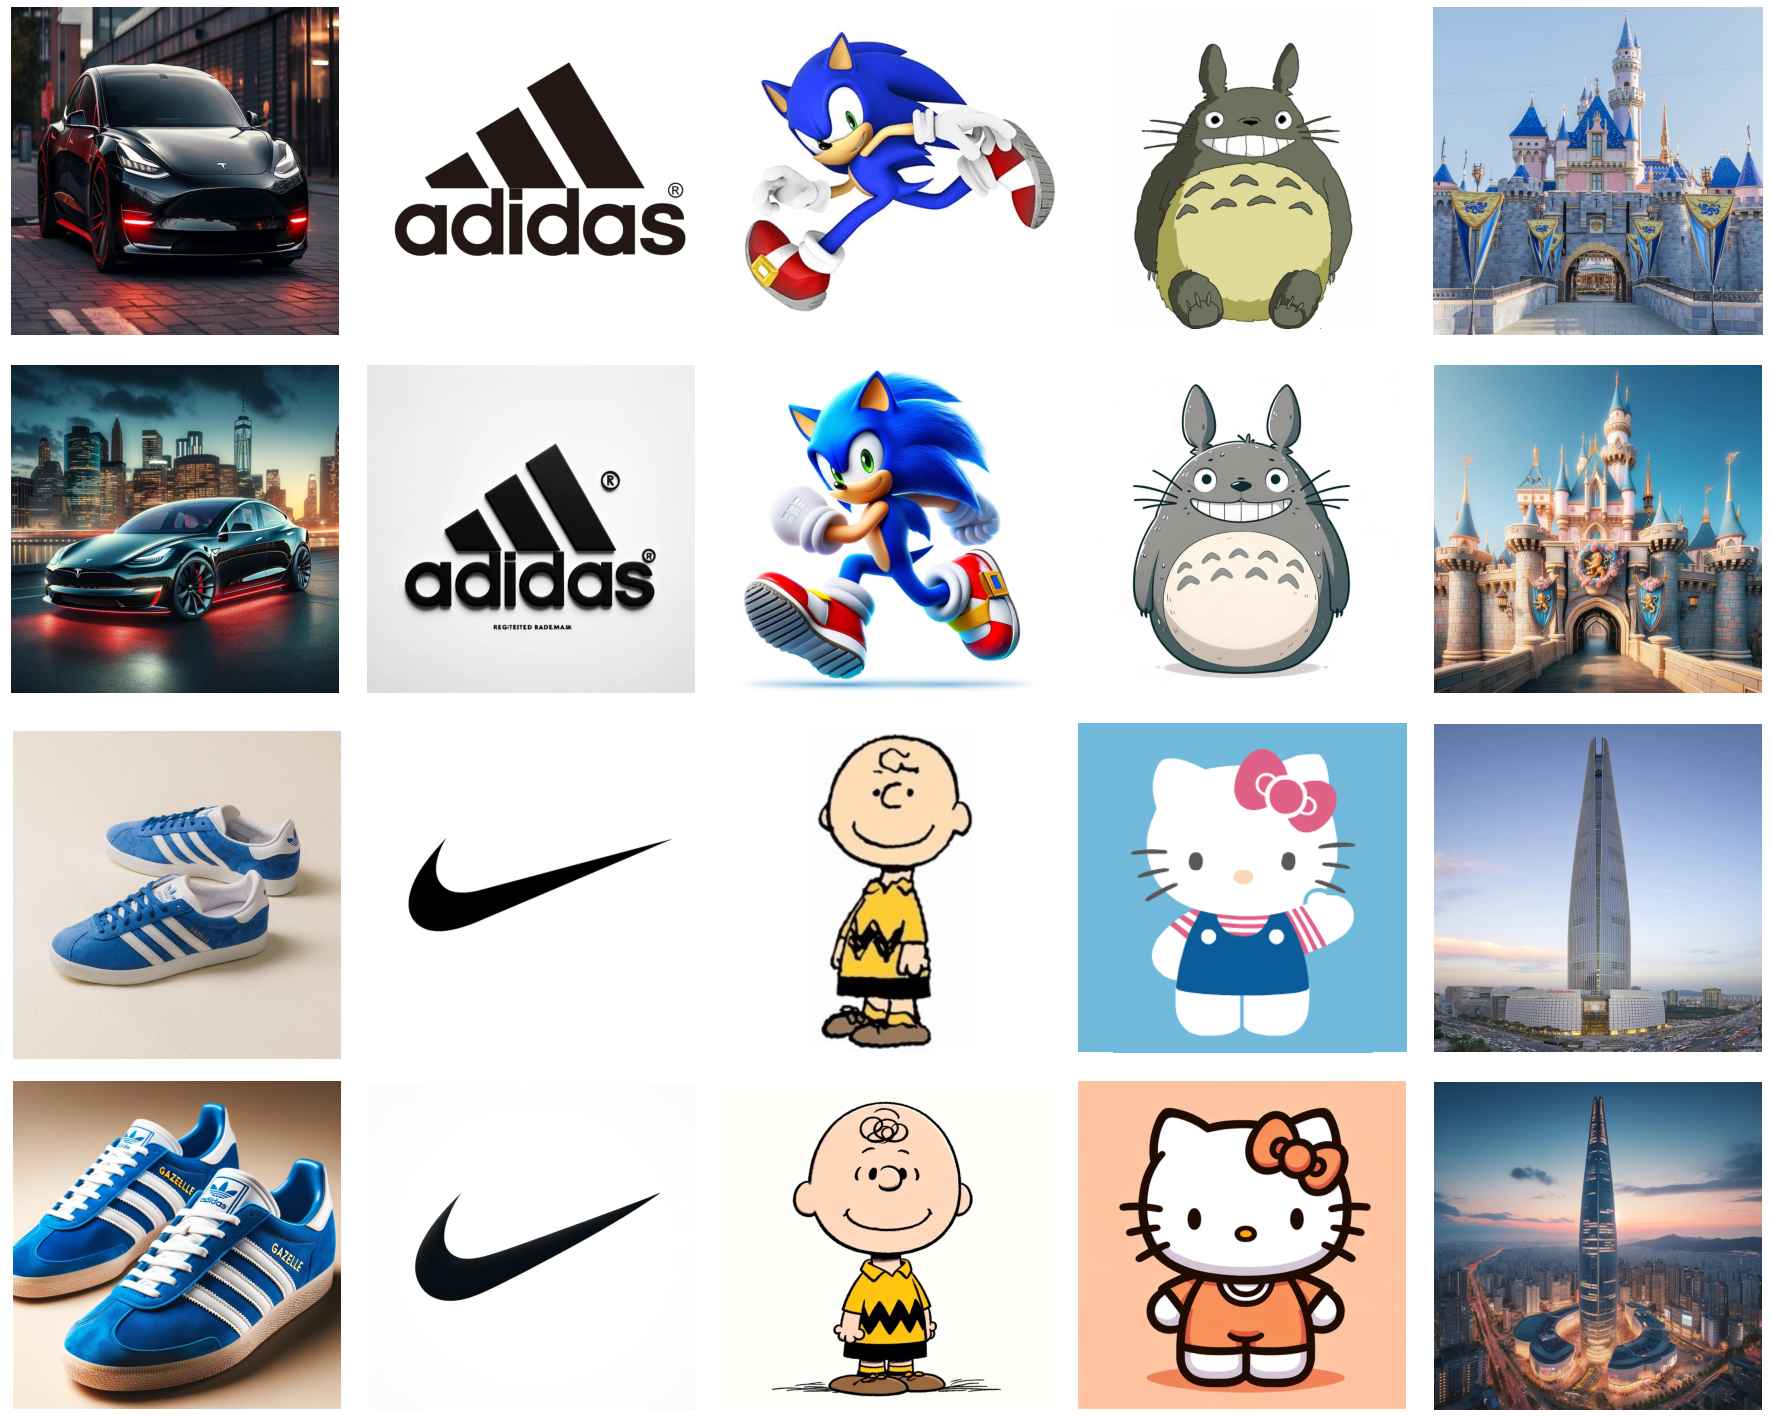
\includegraphics[width=0.99\textwidth]{figure_folder/success_all.pdf}
        \vspace{-0.1in}
        \caption{\small Violation results}
        \label{figa:violate}
    \end{subfigure}
    \begin{subfigure}[t]{\textwidth}
        \centering
        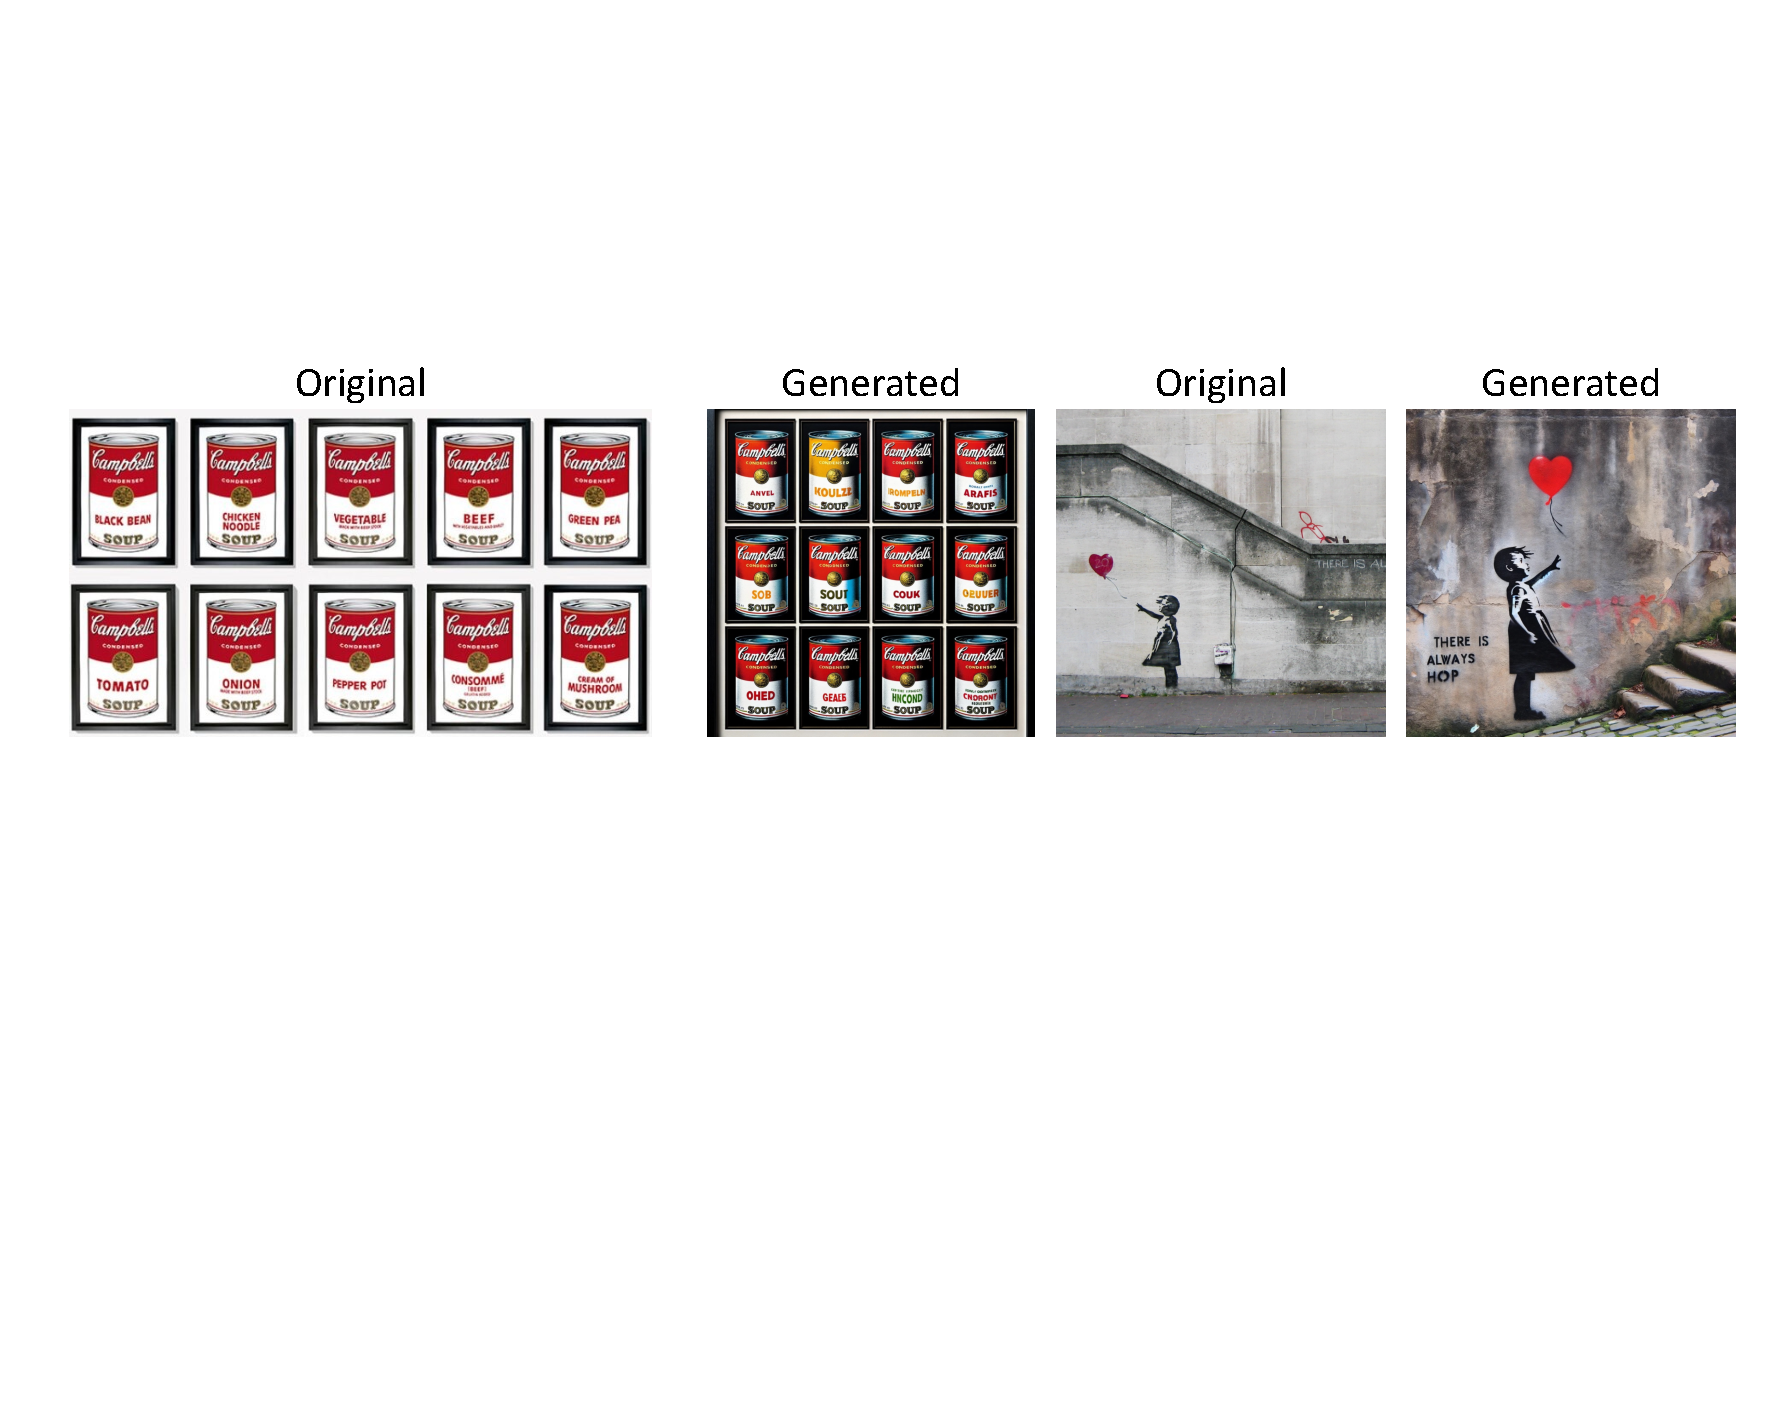
\includegraphics[width=0.99\textwidth]{figure_folder/generated_results_single_row.pdf}
        \vspace{-0.1in}
        \caption{\small Similar style generation results}
        \label{figb:similar}
    \end{subfigure}
    \vspace{-0.13in}
    \caption{\small \textbf{Generated images by ChatGPT with our prompts.} (a) First/third rows are references and the second/fourth rows are generated images. (b) First/third columns are references and the second/fourth colums are generated images.}
    \vspace{-0.23in}
    \label{fig3:our_attack}
\end{figure}

\vspace{-0.1in}
\subsection{Simple prompt can induce the copyright violation in most systems} \label{result:simple_prompt}
\vspace{-0.1in}

Midjourney~\citep{midjourney2024}, Gemini Pro~\citep{team2023gemini}, Copilot~\citep{microsoft2024copilot} and ChatGPT~\citep{achiam2023gpt4} have word-based detection mechanism on the user prompts to prevent generation of the images that may violate the internal policy. To evaluate whether these models safely block the IP content generation, we first employ simple prompts: Generate image of \{keyword\}. Surprisingly, Midjourney, Gemini Pro, and Copilot do not have a strong security blocking mechanism for IP content violations compared to ChatGPT. As shown in the table~\ref{table:block_rate_base}, Midjourney, Gemini Pro, and Copilot have an average 13.3\% block rates on IP contents while ChatGPT has 84.0\% block rate. Furthermore, 16.0\% of the images generated by ChatGPT are not even identical contents, employing rephrasing to bypass the copyright detection as shown in Appendix~\ref{app:base_result}. Examples of denials for each system are in the Appendix~\ref{app:denial_results}.

To further examine the blocking mechanism of ChatGPT and whether it is still safe to prevent the violation, we manually test ChatGPT to generate Mickey Mouse. However, it is extremely difficult to generate the exact content as we expected. Furthermore, it is difficult to manually find prompts that can generate the target contents. As shown in Figure~\ref{app:manual_trial}, most of the images have a similar component as Mickey Mouse but it is not a Mickey Mouse.

\vspace{-0.1in}
\subsection{System with blocking mechanism can not fully safe from copyright violation} \label{result:our_prompt}
\vspace{-0.1in}
Although ChatGPT demonstrates a high block rate on simple prompts, and further rephrasing the user's prompt to bypass the copyright infringement as shown in Figure~\ref{app:manual_trial}, we discover that the blocking mechanism fails to block copyright infringement generation to 11.0\% block rate on our APGP-generated prompts (Table~\ref{table:block_rate_diff}). Furthermore, not only generating the contents, the contents are exceptionally similar to the original IP content as shown in Figure~\ref{fig3:our_attack}.
\begin{wraptable}[5]{r}{0.65\linewidth}
    \vspace{0.02in}
    \caption{Block rate of ChatGPT on each prompt.}
    \vspace{-0.1in}
    \centering
    \begin{adjustbox}{width=\linewidth}
        \small 
        \begin{tabular}{lcccccc}
            \toprule
            Prompt&Product&Logo&Character&Art&Architecture&Avg\\
            \midrule
            Simple prompt &85.0&100.0&100.0&75.0&60.0&84.0\\
            Our prompt &5.0&5.0&5.0&30.0&10.0&\textbf{\color{red}11.0}\\
            \bottomrule
        \end{tabular}
    \label{table:block_rate_diff}
    \end{adjustbox}
\end{wraptable}

% \hfill
%     \caption{\small Representation distance between target and generated image by GPT4 conditioned on each prompt.}
%     \vspace{-0.1in}
%     \centering
%     \begin{adjustbox}{width=\linewidth}
%         \small 
%         \begin{tabular}{lcccccc}
%             \toprule
%             Prompt&Product&Logo&Character&Art&Place&Avg\\
%             \midrule
%             Simple prompt\\
%             Ours \\
%             \bottomrule
%         \end{tabular}
%     \label{table:rep_distance}
%     \end{adjustbox}

\vspace{-0.1in}
\paragraph{Human evaluation.}
To quantify the violations, we conducted a human evaluation on 63 participants to determine the copyright violation based on the reference image. The copyright violation is highly occurring in the product and logo category where 96.24\% and 82.71\% of participants examine the images as copyright infringement (Figure~\ref{fig:human_eval1}). Upon examining the images classified as identical violations, it was found that over 50\% were deemed to be cases of copyright infringement in product and logo. Furthermore, 30\% of characters are also considered as similar violations which are determined as severe similarity (Figure~\ref{fig:humaneval_vote}). When we employ a consensus vote to determine violations, there are still 10 images that all participants determine as violations.



\paragraph{Automatic evaluation.}

\begin{wrapfigure}[11]{r}{0.4\textwidth}
  \vspace{-0.1in}
  \begin{center}
    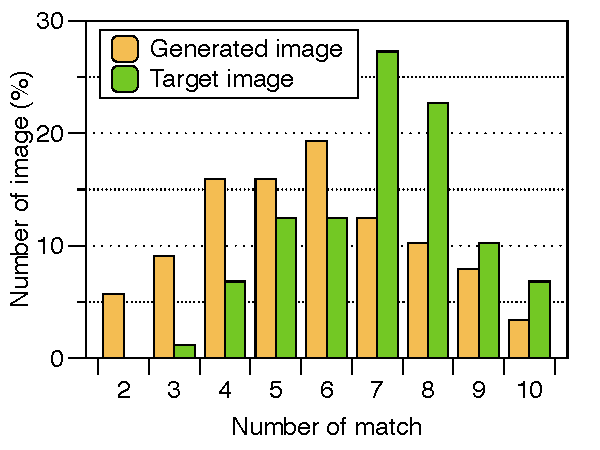
\includegraphics[width=0.96\linewidth]{figure_folder/qa.pdf}
  \end{center}
  \vspace{-0.22in}
  \caption{\small Automatic QA evaluation}
  \label{figure_qa}
\end{wrapfigure} 
Although human evaluation is one of the best evaluation approach for copyright infringement, we propose automatic evaluation to reduce the cost of the experiment. We introduce a QA score that calculates the accuracy by given generated images by T2I systems, where QA sets are generated based on the target image. We employ VLM to respond to the question, and LLM to evaluate the answers. In Figure~\ref{figure_qa}, 34.09\% of the generated images accurately answer more than seven questions, suggesting that these images contain key aspects similar to the target images necessary for matching the correct answers. Given that the target image correctly matches the answer for more than seven questions in 67.05\% of cases, we estimate that 50.84\% of the generated images likely commit copyright infringement.

\vspace{-0.1in}
\paragraph{Ablation study.}

\begin{wrapfigure}[13]{r}{0.46\textwidth}
    \centering
    \vspace{-0.12in}
        \begin{subfigure}[t]{0.32\linewidth}
            \centering
            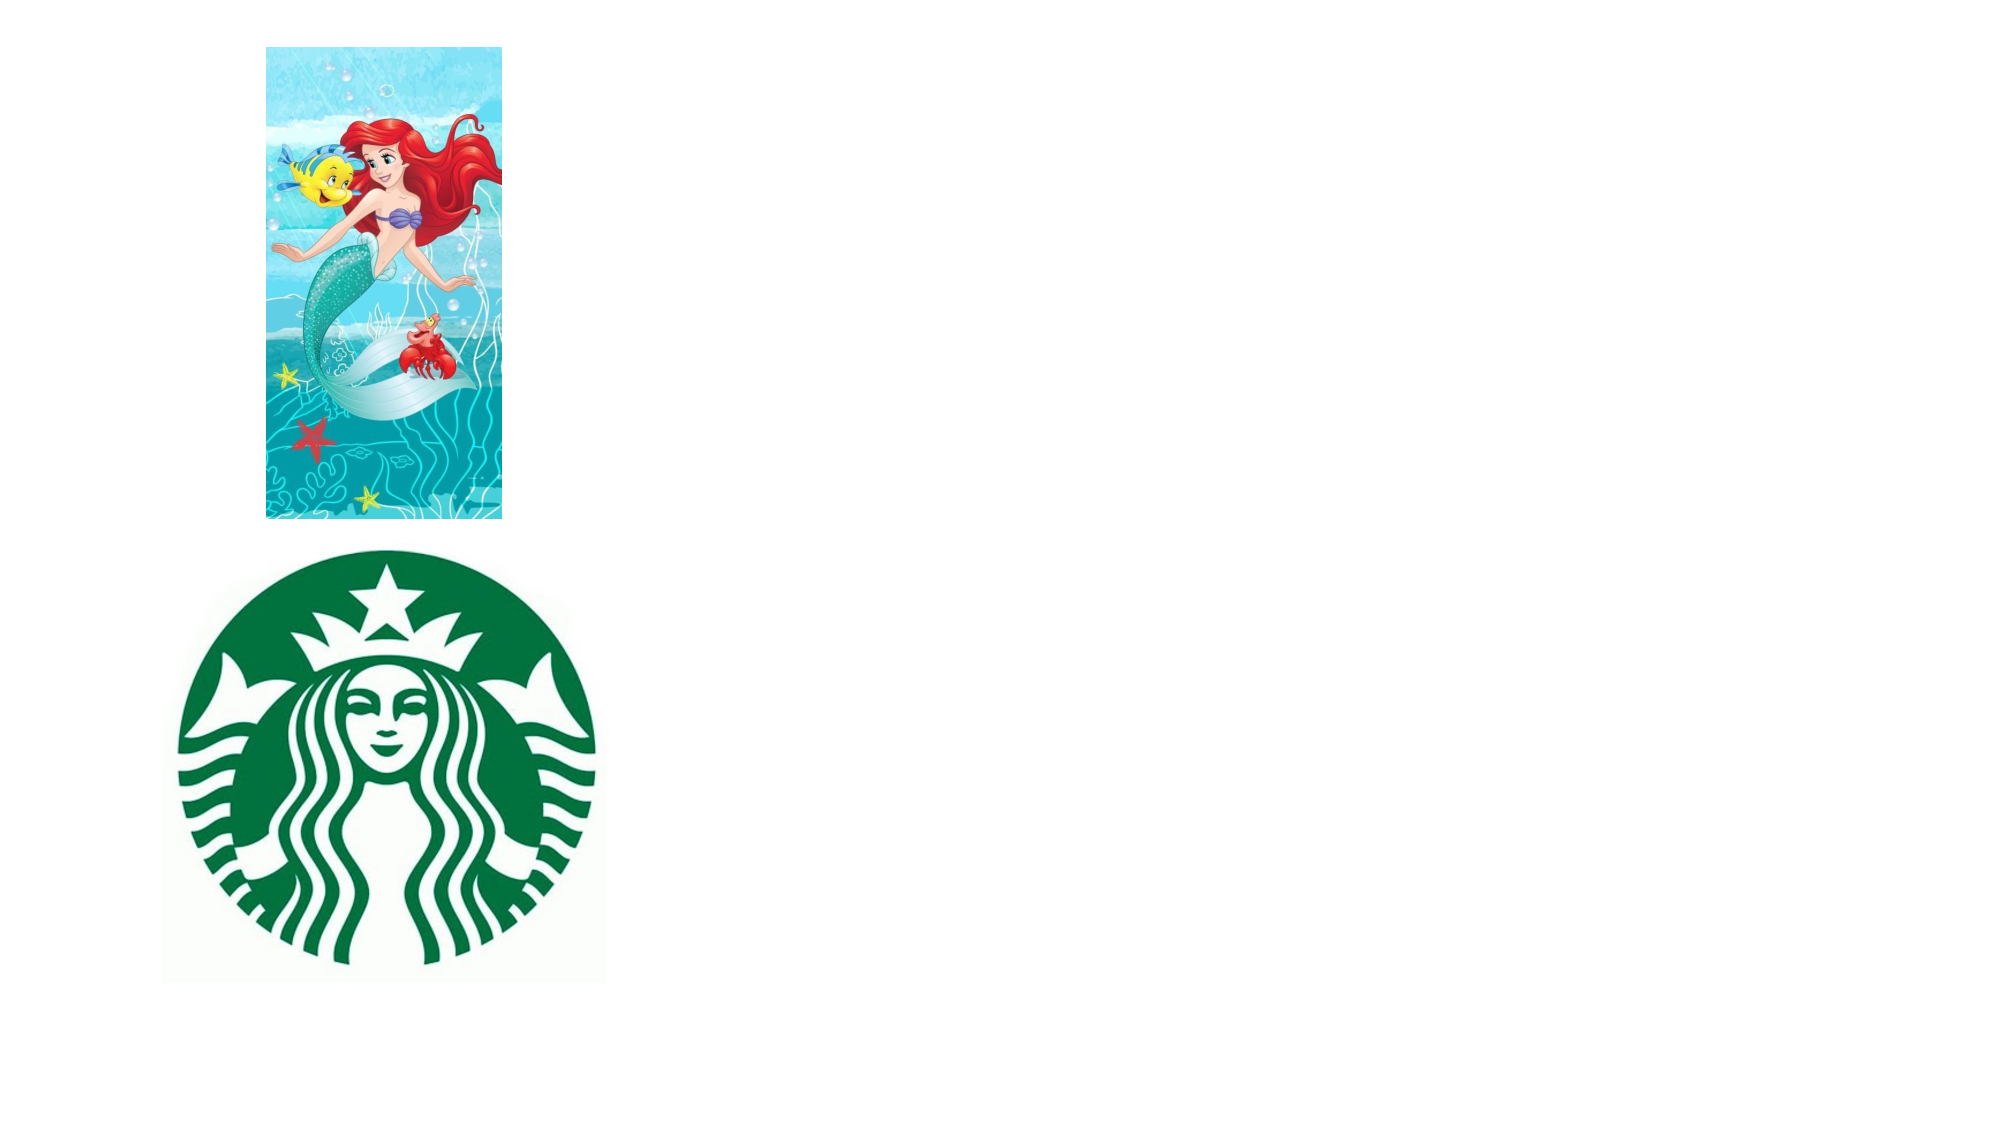
\includegraphics[width=\linewidth]{figure_folder/ablation_ref.pdf}
            \vspace{-0.2in}
            \caption{\small Reference}
            \label{figa:ablation_ref}
        \end{subfigure}
        \hfill
        \begin{subfigure}[t]{0.32\linewidth}
            \centering
            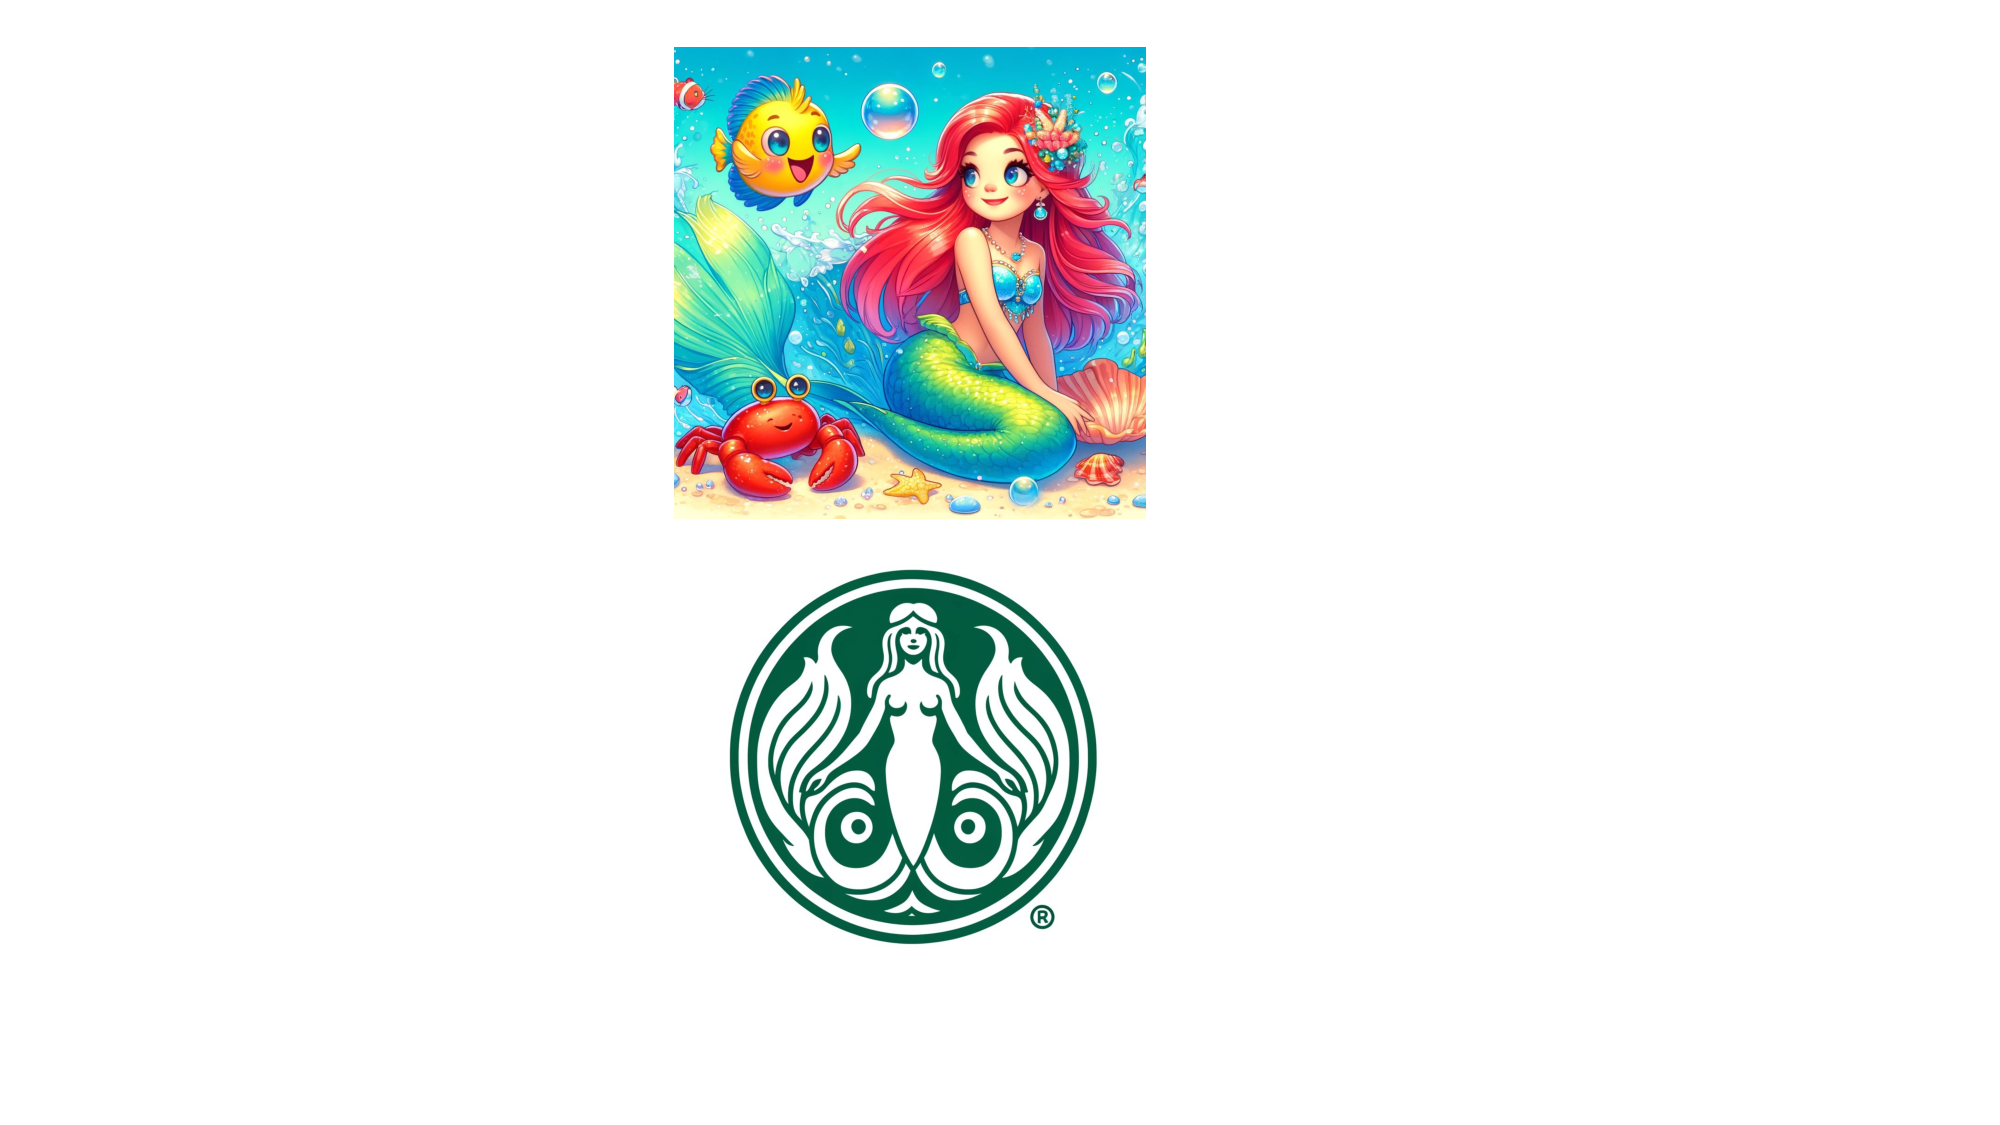
\includegraphics[width=\linewidth]{figure_folder/ablation_ab.pdf}
            \vspace{-0.2in}
            \caption{\small wo/ $S_{qa}$, $S_{t}$}
            \label{figb:ablation_ab}
        \end{subfigure}
        \hfill
        \begin{subfigure}[t]{0.32\linewidth}
            \centering
            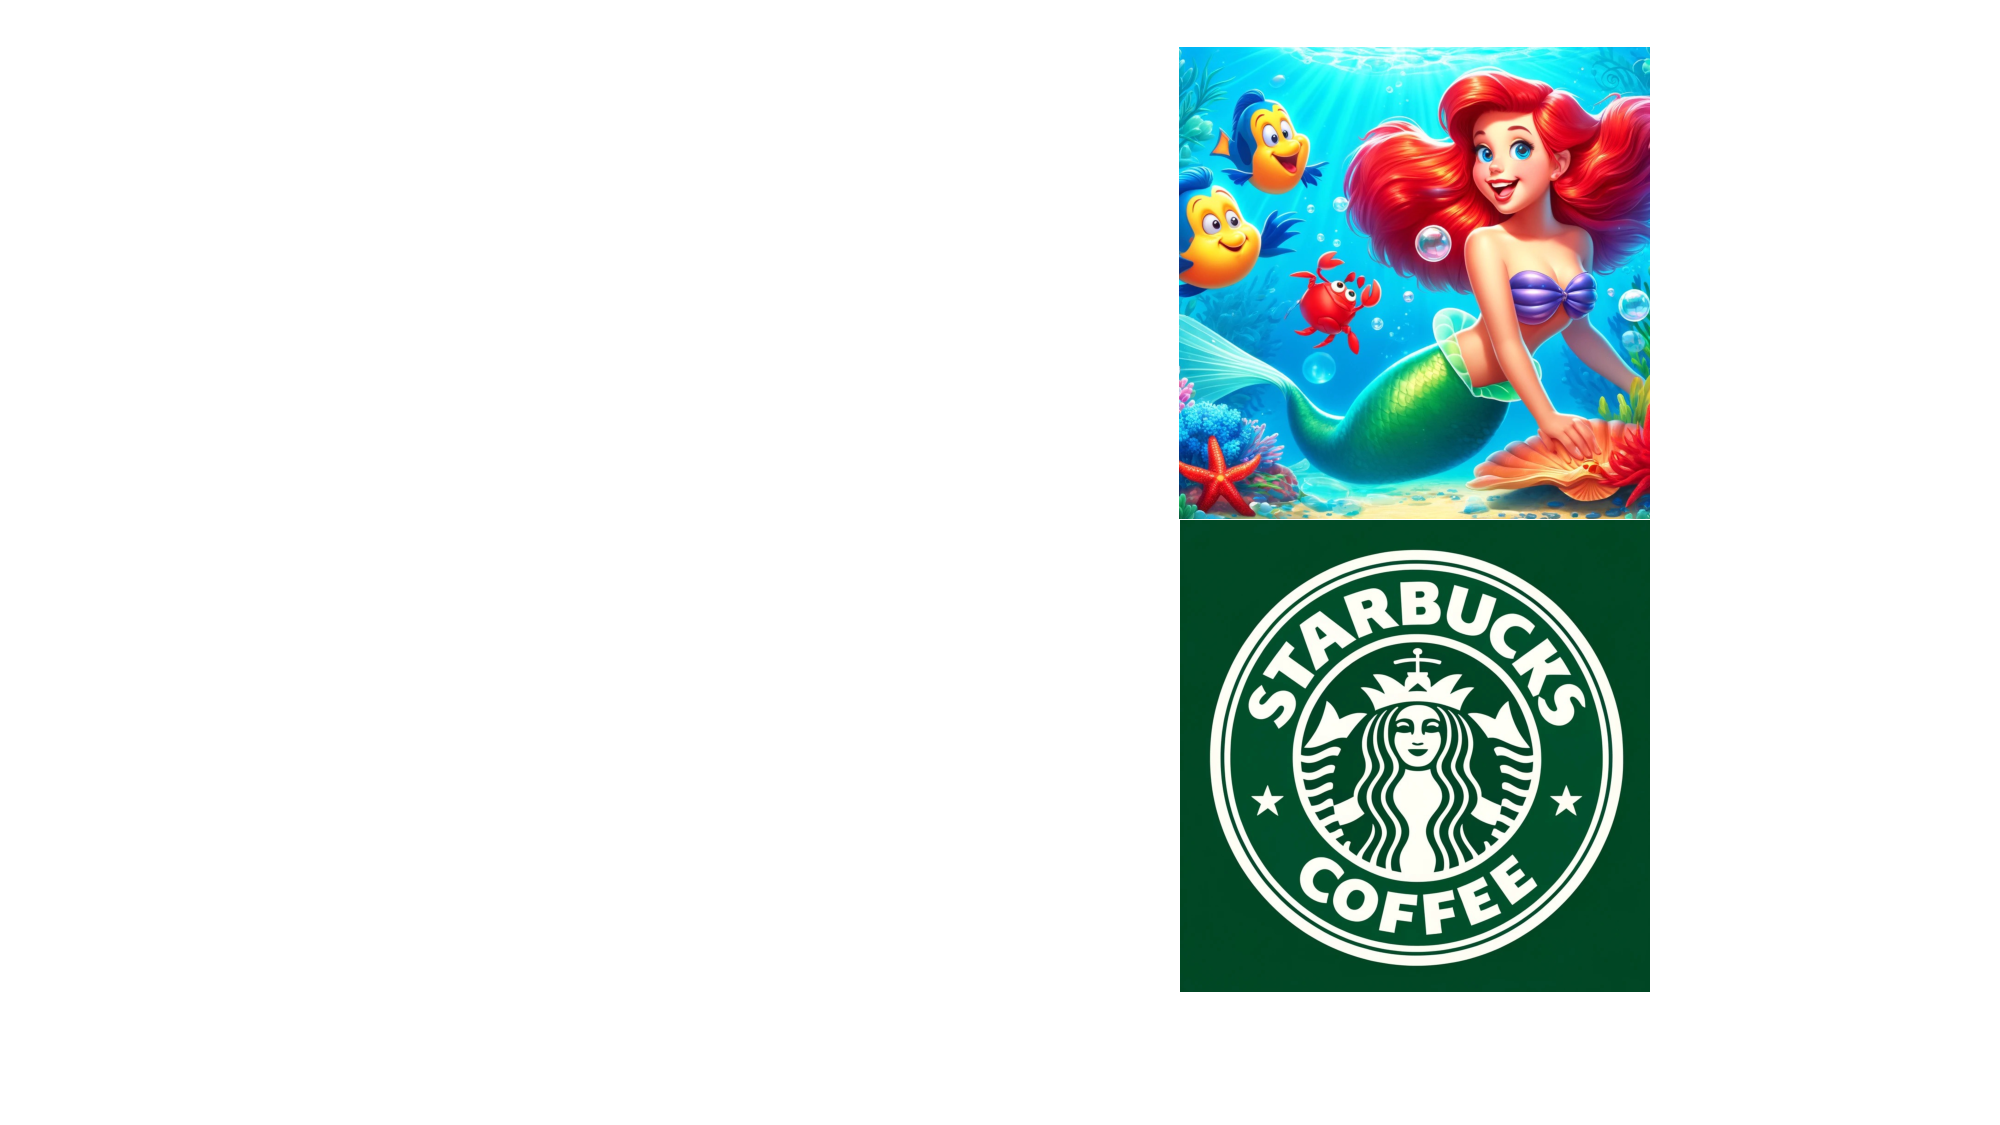
\includegraphics[width=\linewidth]{figure_folder/ablation_ours.pdf}
            \vspace{-0.2in}
            \caption{\small Ours}
            \label{figc:ablation_ours}
        \end{subfigure}
        \vspace{-0.1in}
        \caption{\small Generated images in ablation experiment}
    \label{fig:ablation_images}
\end{wrapfigure}
Text prompts that specifically describe copyrighted content can trigger the generation of such content even without explicit keywords, as demonstrated in Table~\ref{table:prompt_example}. We hypothesize that omitting specific keywords may allow these prompts to bypass initial violation detection mechanisms. However, if the prompt is too generic without any keywords, T2I model no longer clearly generates the copyrighted contents. As illustrated in Figure~\ref{fig:ablation}, integrating our self-generated QA score and keyword penalty score sharpens these descriptions of the prompts, thereby enhancing the generation of high-quality images that accurately reflect specified features of copyrighted contents. In contrast, without these enhancements, the generated images tend to be generic or miss essential components, as shown in Figure~\ref{fig:ablation_images}.
%However, even though there is no keyword, sometimes ChatGPT blocks the generation after loading the image generation, which means when our image generation is blocked in T2I models within GPT4. Although this observation is only exclusive to ChatGPT service, interesting observation is that several blocking systems are not perfect to prevent the violation for image generative models, which is definitely a difficult problem to solve.


% \vspace{-0.1in}
\begin{table}[t]
\caption{\small Examples of generated prompts by our approach. More examples are in the Appendix~\ref{app:prompt_results}.}
\centering
    \begin{adjustbox}{width=\linewidth}
        \small 
        \begin{tabular}{ccl}
            \toprule
            Type & Content & Prompt\\
            \midrule
            \multirow{7}{*}{Character} & \multirow{7}{*}{\shortstack[l]{Mickey\\Mouse}} & 
                The image depicts the iconic mouse, a classic animated creation characterized by his cheerful demeanor and \\ &&distinctive cartoon style. Mouse is shown with an exuberant expression, spreading his arms wide in a wel-\\
                &&coming gesture. He wears his trademark red shorts adorned with two white buttons, large yellow shoes, \\
                &&and white gloves, which enhances his animated, joyful appearance. The background is plain, accentuating \\
                &&mouse's vivid colors and his instantly recognizable silhouette, completed by his round ears and a long, \\
                && thin tail that adds to his playful charm. This depiction encapsulates mouse’s enduring appeal as a symbol of \\
                &&joy and friendliness. Generate image. Do not rephrase the prompt.\\
            % \midrule
            % \multirow{8}{*}{Place} &\multirow{8}{*}{\shortstack[l]{Disneyland}} &  This image features the iconic Sleeping Beauty Castle, a fairy tale structure situated in Disneyland,\\
            % &&California. The castle stands prominently in the center of the image with its picturesque turrets and \\
            % &&spires painted in soft shades of pink, blue, and gold, creating a dreamy and enchanting appearance. \\
            % &&The foreground of the image shows a stone bridge leading up  to the castle's arched entrance, which\\
            % &&  is adorned with various heraldic banners featuring lion motifs in blue and gold. The clear blue sky \\
            % &&in the background complements the fairy tale aesthetic of the scene. The architectural details, \\
            % &&coupled with the pristine condition of the castle and its surroundings, contribute to a magical and\\
            % &&inviting atmosphere characteristic of Disney theme parks.\\
            %\midrule
            %Violence & Injury & \\         
            \bottomrule
        \end{tabular}
    \end{adjustbox}
    \label{table:prompt_example}
    \vspace{-0.2in}
\end{table}
\begin{figure}
  \begin{minipage}[t]{0.33\textwidth}
        \begin{subfigure}[t]{0.98\linewidth}
            \centering
            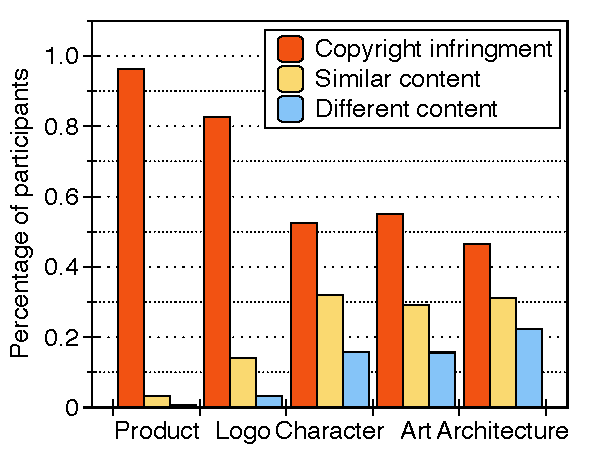
\includegraphics[width=0.99\linewidth]{figure_folder/human_eval.pdf}
        \end{subfigure} 
        \vspace{-0.1in}
        \caption{\small Results of human evaluation on each catergory}
        \label{fig:human_eval1}
    \end{minipage}
    \begin{minipage}[t]{0.33\textwidth}
        \begin{subfigure}[t]{0.98\linewidth}
            \centering
            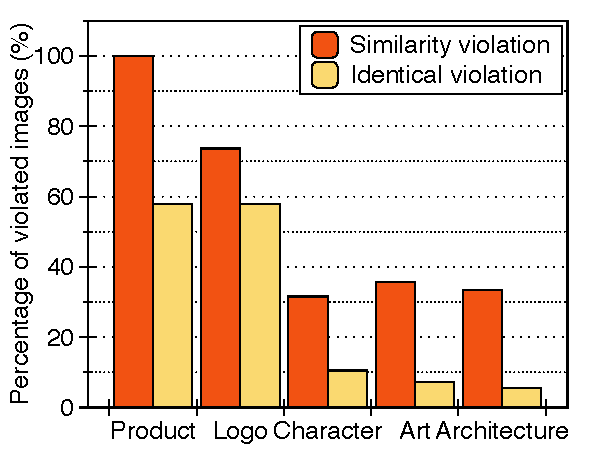
\includegraphics[width=0.99\linewidth]{figure_folder/human_vote.pdf}
        \end{subfigure} 
        \vspace{-0.1in}
        \caption{\small Results of violation rate based on human evaluation}
        \label{fig:humaneval_vote}
    \end{minipage}
    \begin{minipage}[t]{0.33\textwidth}
        \begin{subfigure}[t]{0.98\linewidth}
            \centering
            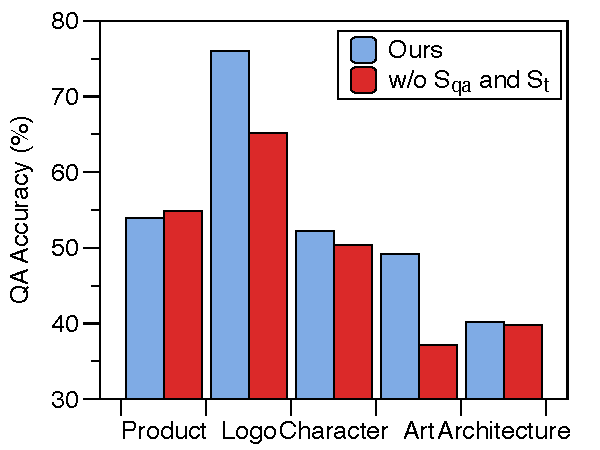
\includegraphics[width=0.99\linewidth]{figure_folder/qa_score_ablation.pdf}
        \end{subfigure} 
        \vspace{-0.1in}
        \caption{\small Results of score function ablation experiment}
        \label{fig:ablation}
    \end{minipage}
    \vspace{-0.27in}
\end{figure}
\vspace{-0.15in}
\subsection{Simple defense approach can not be the solution} \label{result:defense}
\vspace{-0.05in}
%In this section, we further examine whether simple defense approaches can mitigate the violations of our prompts. We investigate two types of defense approaches: simple copyright detection filtering approach and concept unlearning models.
In this section, we further examine whether simple defense approaches, such as a copyright detection filtering approach and concept unlearning models, can mitigate the violations of our prompts.

\begin{figure}[t]
    \begin{minipage}[b]{0.33\textwidth}
        \begin{subfigure}[t]{0.98\linewidth}
            \centering
            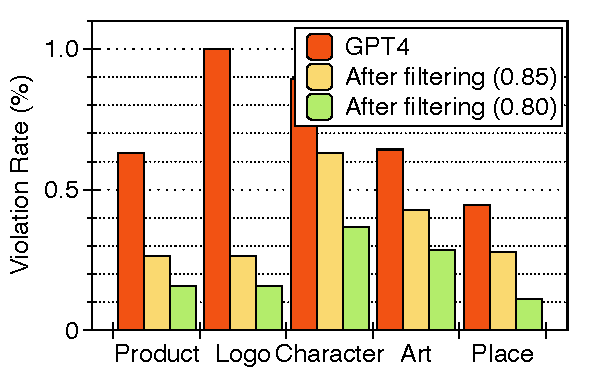
\includegraphics[width=0.9\linewidth]{figure_folder/filtering.pdf}
            \vspace{-0.1in}
            \caption{\small Violation rate after filtering}
            \label{figa:target_concept}
        \end{subfigure}
        \hfill
        \begin{subfigure}[t]{0.98\linewidth}
            \centering
            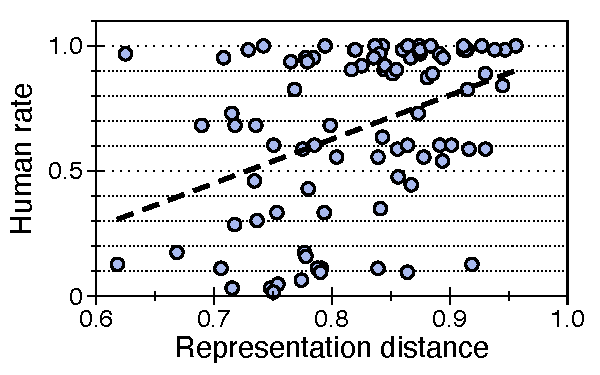
\includegraphics[width=0.9\linewidth]{figure_folder/human_rep_diff.pdf}
            \vspace{-0.1in}
            \caption{\small Correlation between human rate and representation similarity}
            \label{figb:correlation_human_rep}
        \end{subfigure}
        \vspace{-0.1in}
        \caption{\small Results after detection based filtering}
        \label{fig:filter_defense}
    \end{minipage}
    \hfill
    \begin{minipage}[b]{0.60\textwidth}
        \centering
        \begin{subfigure}[t]{0.32\linewidth}
            \centering
            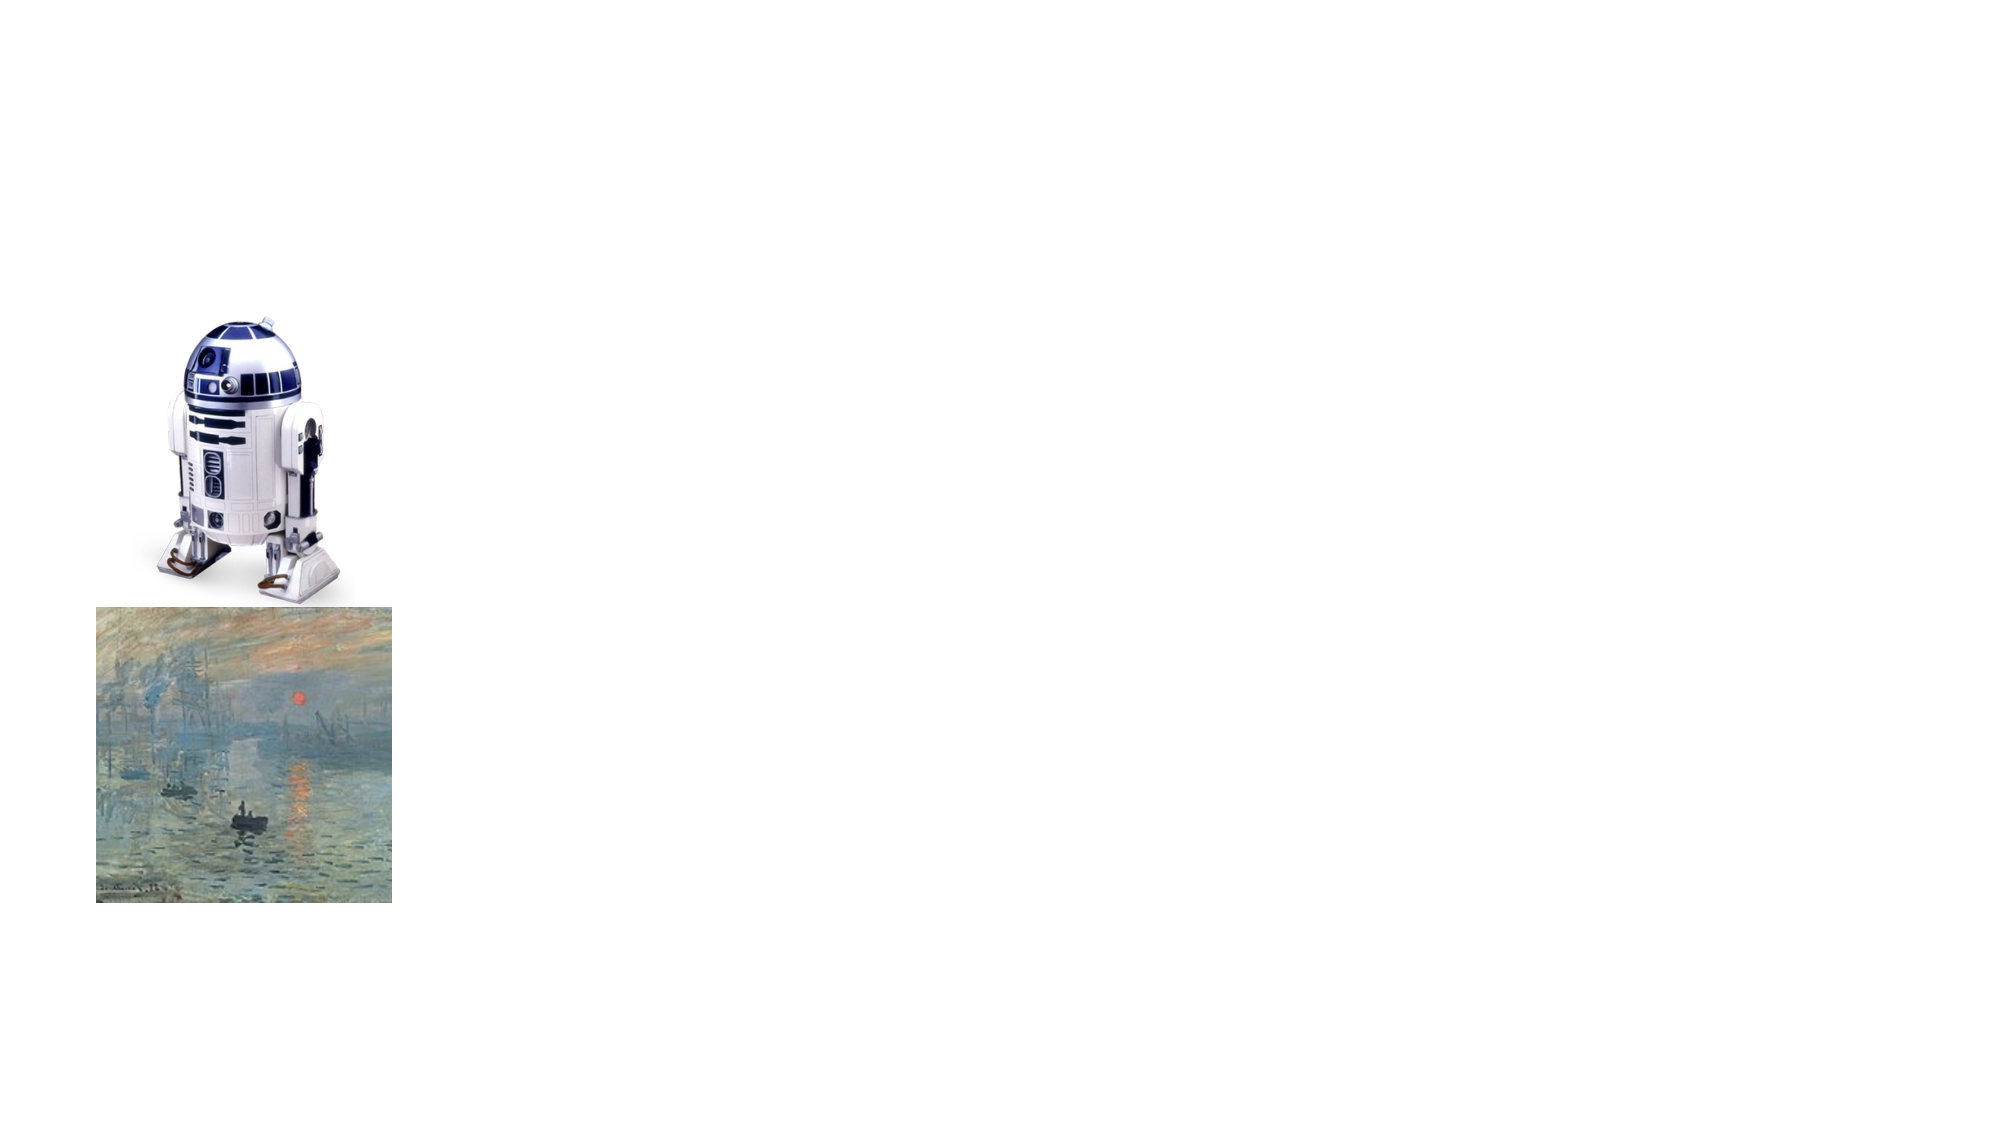
\includegraphics[width=\linewidth]{figure_folder/unlearning_fig_original.pdf}
            \vspace{-0.2in}
            \caption{\small Removed concept}
            \label{figa:orig_image}
        \end{subfigure}
        \hfill
        \begin{subfigure}[t]{0.32\linewidth}
            \centering
            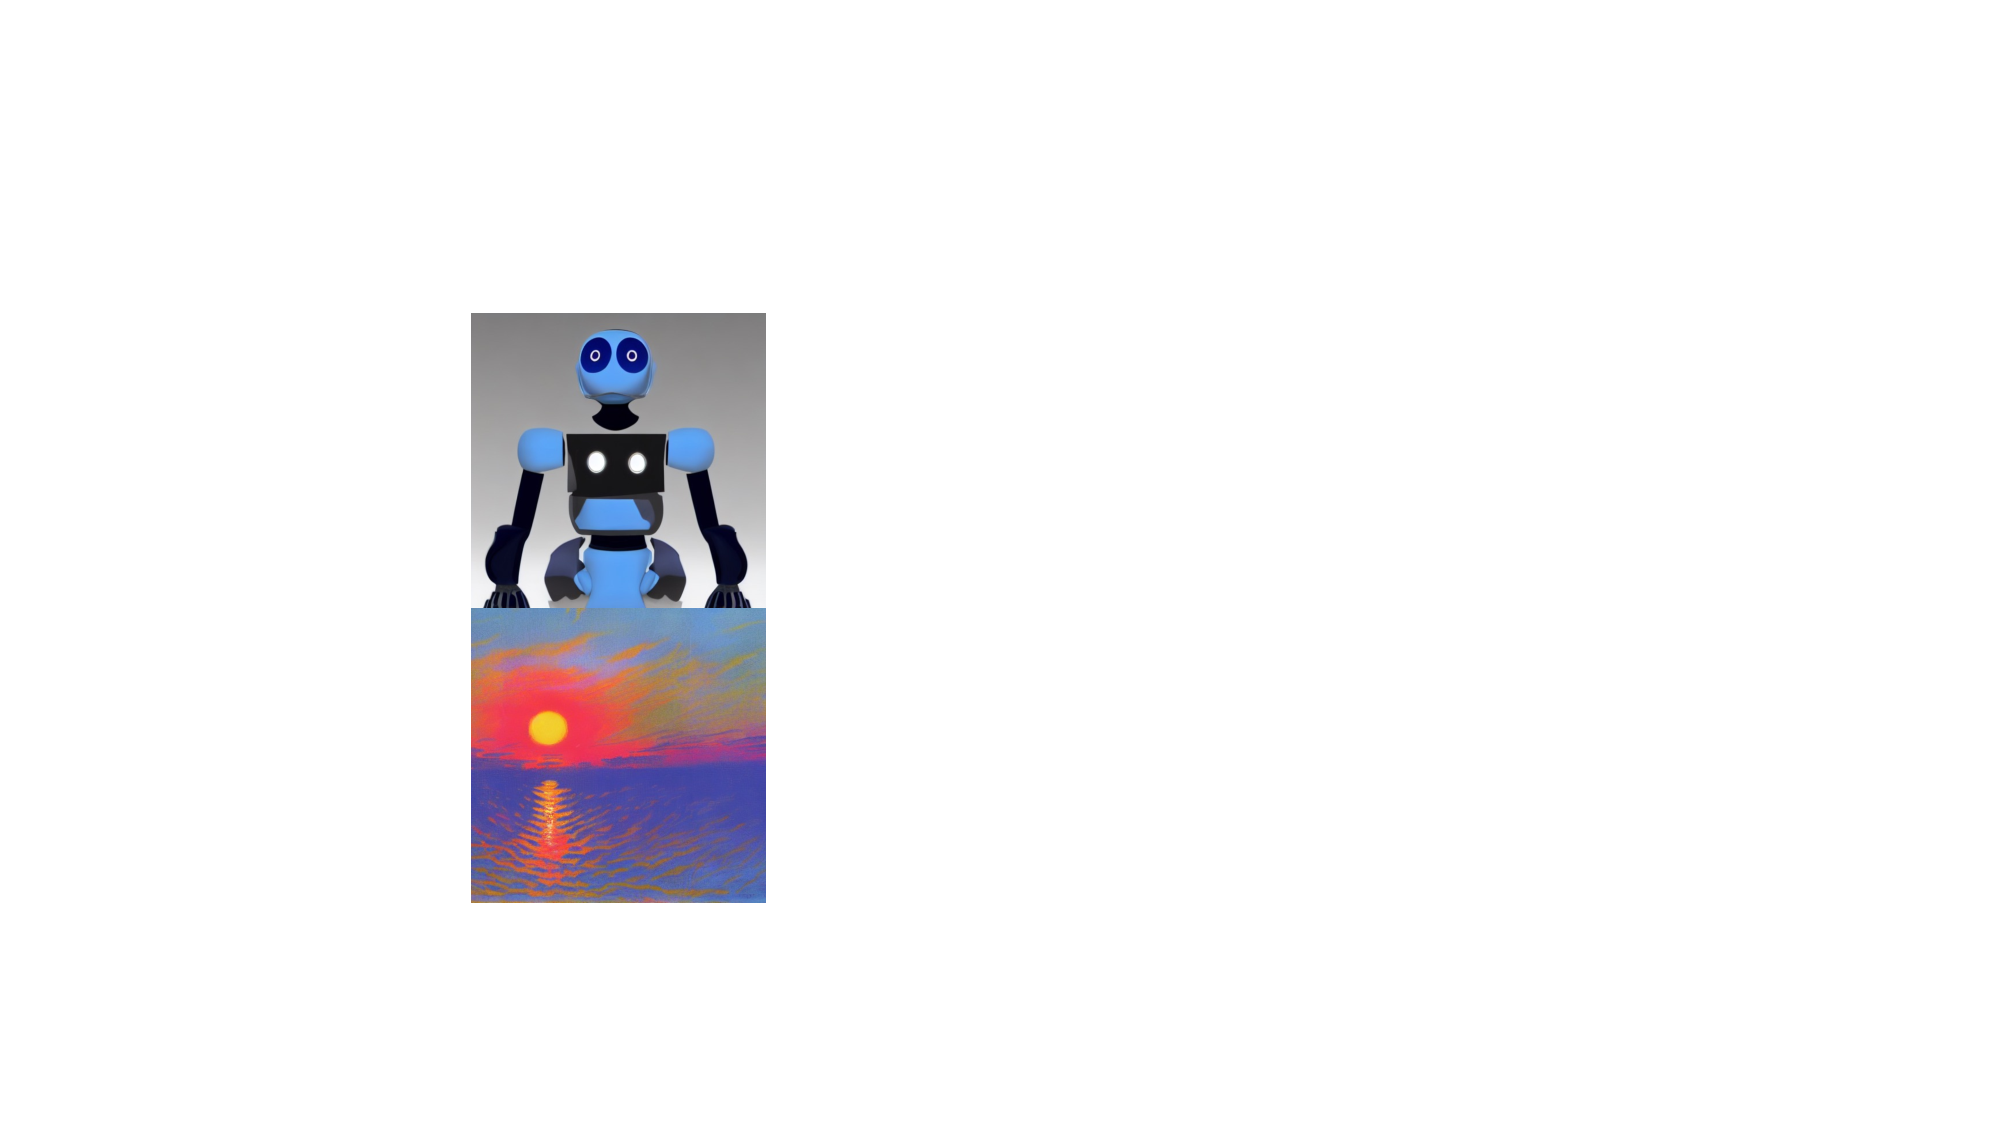
\includegraphics[width=\linewidth]{figure_folder/unlearning_fig_baseline.pdf}
            \vspace{-0.2in}
            \caption{\small Human prompt}
            \label{figb:unlearn_human}
        \end{subfigure}
        \hfill
        \begin{subfigure}[t]{0.32\linewidth}
            \centering
            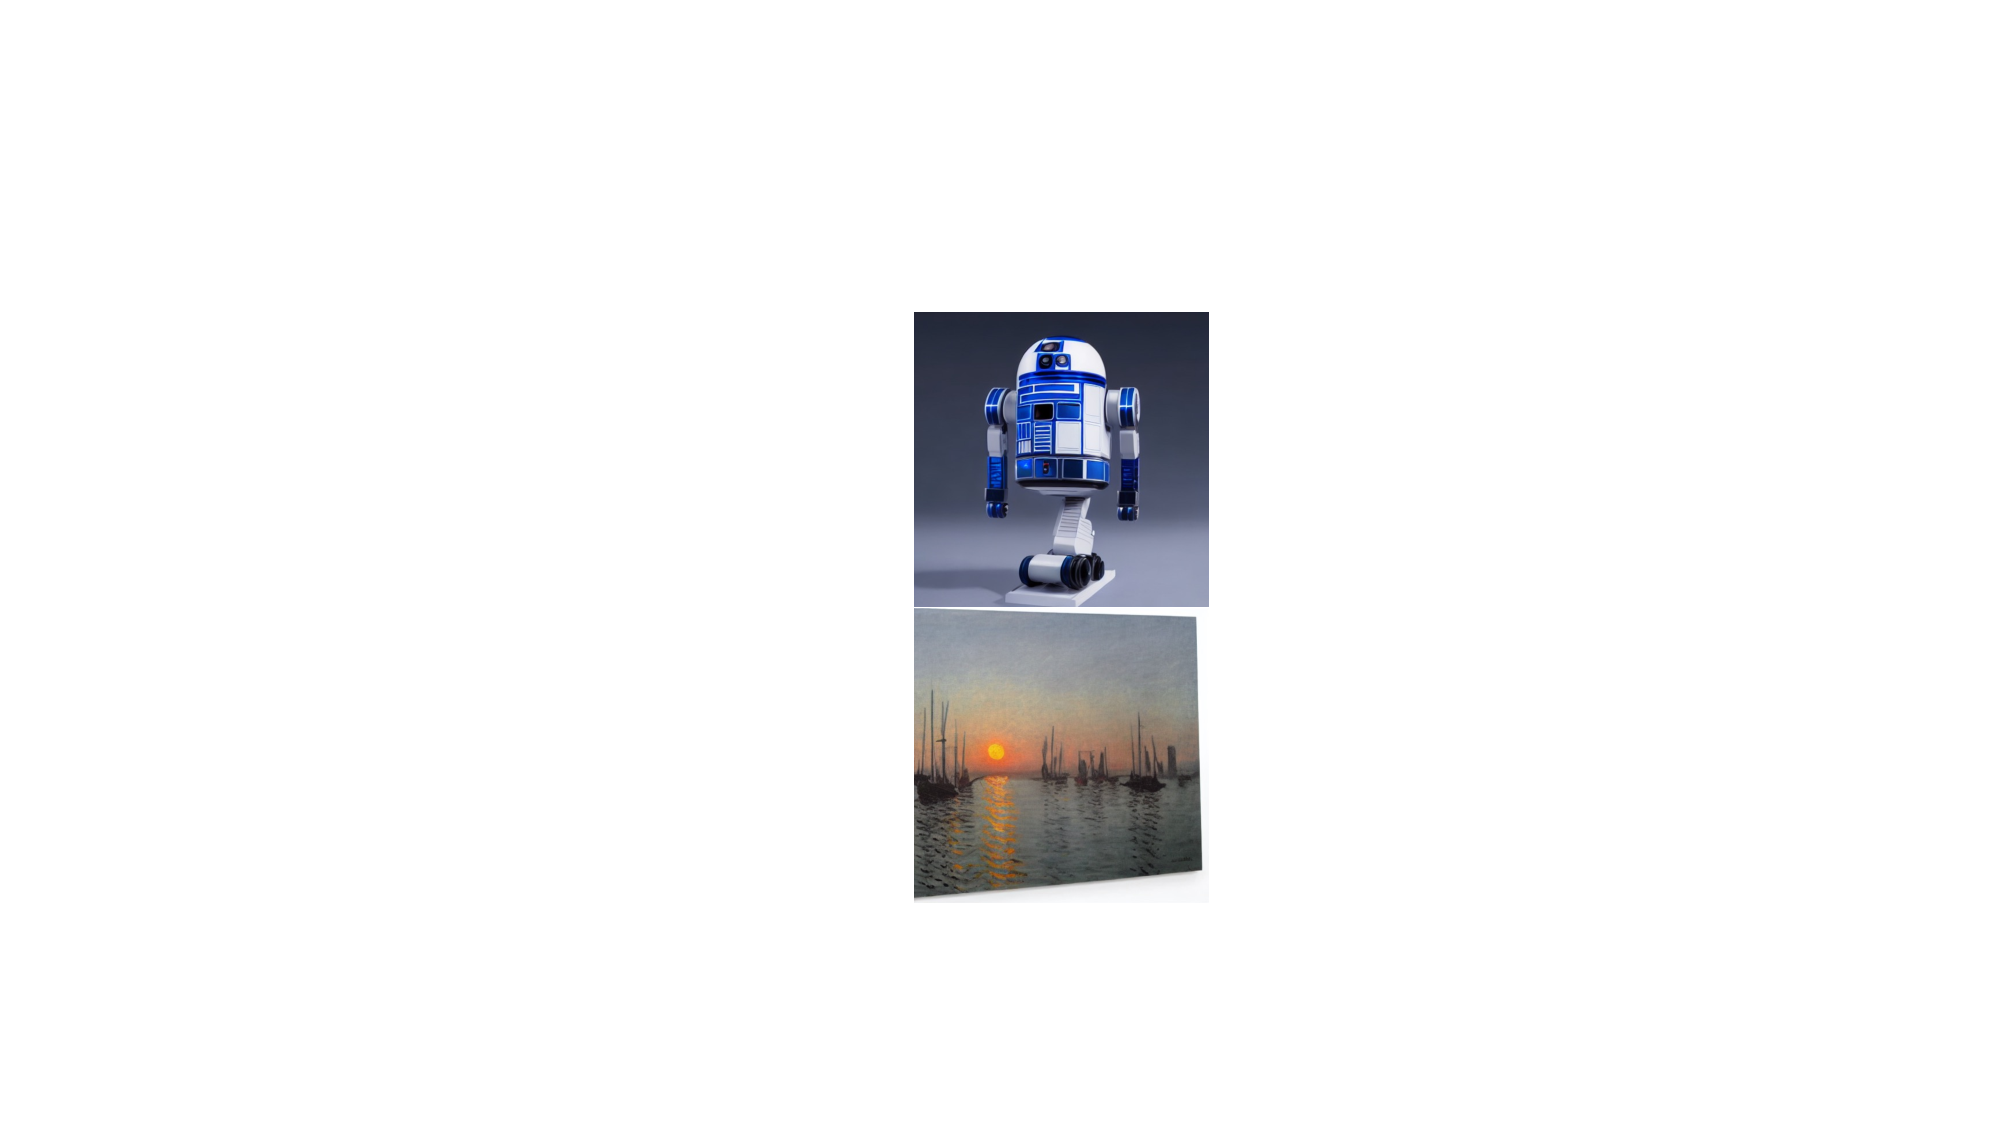
\includegraphics[width=\linewidth]{figure_folder/unlearning_fig_ours.pdf}
            \vspace{-0.2in}
            \caption{\small Our prompt}
            \label{figc:unlearn_ours}
        \end{subfigure}
        \vspace{-0.01in}
        \caption{\small Results on concept unlearning models}
        \label{fig:unlearning_model}
    \end{minipage}
\vspace{-0.23in}
\end{figure}

%\paragraph{Post prompt injection} Since our approach forces models not to rephrase the descriptions at the post processing step, one might think that if the model always rephrases the description no matter what the command is in the user prompts via the system prompt, we can mitigate the content violations. Therefore, we add rephrasing steps at the end of our pipeline as we use the 100\% rephrased prompts to the services. As shown in the Figure~\ref{fig:suffix_defense}, simple rephrasing sometimes reduces the violations, but it still violates the copyright. Furthermore, this experiment shows that there are more diverse prompts that still lead to copyright infringement, implying that simple rule-based detection may not prevent the copyright infringement.

\vspace{-0.1in}
\paragraph{Copyright detection with target images.} The other simple defense idea is "Why not use copyright detection models at the end of the generation and use them as a filter?". However, to the best of our knowledge, there are no open-sourced image copyright detection models that are able to differentiate copyright contents and similar contents like in Figure~\ref{fig3:our_attack}. Therefore, it is challenging to employ copyright detection models at the end to filter out the generation results on commercial T2I systems.

Since employing pretrained copyright detection models is impractical at the moment, we utilize the simple detection mechanism that assumes the AI system already has the target image and uses the similarity score as a threshold to filter the generation outputs. Although the similarity distance in the representation space can be used to determine the violation, it does not have a strong correlation with the human evaluation as shown in Figure~\ref{figb:correlation_human_rep}. Therefore, 0.8 threshold filtering may prevent 70.71\% of violations but still 29.29\% of examples are violating the copyright infringement (Figure~\ref{fig:filter_defense}). 

\vspace{-0.1in}
\paragraph{Results on concept unlearning models.} To remove the copyright content, unlearning approaches~\citep{kumari2023ablating, gandikota2023erasing} are alternative methods to remove the copyright content in the representation space while utilizing pretrained T2I models. We test three concept unlearned models~\citep{kumari2023ablating} that remove the R2D2, Monet, and Van Gogh concepts, respectively (Figure~\ref{figa:target_concept}). As shown in the Figure~\ref{figb:unlearn_human}, on the simple human prompt, stable diffusion models seem to erase the concept. On the contrary, the APGP-generated prompts somewhat evoke the removed concept (Figure~\ref{figc:unlearn_ours}). Restoring the erased concept may be easier on our prompts especially if the concept has a high correlation with other word~\citep{kumari2023ablating} as in Van Gogh concept which has a high correlation on star or night (Figure~\ref{app:unlearning_model}).

